\documentclass[11pt,a4paper,twoside]{article}

% LaTeX-Umsetzung der "Richtlinien für Projekt- und Diplomarbeiten"
% der LFE Medieninformatik, LMU München. (Autor: Richard Atterer, 27.9.2006, 23.10.2007), Bug-Fixing Mark Kaczkowski (23.6.2008)

\usepackage[T1]{fontenc} % sonst geht \hyphenation nicht mit Umlauten
%\usepackage[latin1]{inputenc} % man kann schreiben äöüß statt "a"o"u"s
\usepackage[utf8]{inputenc} % wie oben, aber UTF-8 als Encoding statt ISO-8859-1 (latin1)
\usepackage[ngerman,british]{babel} % deutsche Trennregeln, "Inhaltsverzeichnis" etc.
%\usepackage{ngerman} % Alternative zum Babel-Paket oben
\usepackage{mathptmx} % Times-Roman-Schrift (auch für mathematische Formeln)
\usepackage{multicol} % Mehrspaltigkeit im Anhang
\usepackage{hyphenat} % Um Worttrennungen unterdrücken zu können
\usepackage{pbox}

% Zum Setzen von URLs
\usepackage{color}
\definecolor{darkred}{rgb}{.25,0,0}
\definecolor{darkgreen}{rgb}{0,.2,0}
\definecolor{darkmagenta}{rgb}{.2,0,.2}
\definecolor{darkcyan}{rgb}{0,.15,.15}
\usepackage[plainpages=false,bookmarks=true,bookmarksopen=true,colorlinks=true,
  linkcolor=darkred,citecolor=darkgreen,filecolor=darkmagenta,
  menucolor=darkred,urlcolor=darkcyan]{hyperref}

% pdflatex: Bilder in den Formaten .jpeg, .png und .pdf
% latex: Bilder im .eps-Format
\usepackage{graphicx}

\usepackage{fancyhdr} % Positionierung der Seitenzahlen
\fancyhead[LE,RO,LO,RE]{}
\fancyfoot[CE,CO,RE,LO]{}
\fancyfoot[LE,RO]{\Roman{page}}
\renewcommand{\headrulewidth}{0pt}
\setlength{\headheight}{13.6pt} % behebt headheight Warning

% Korrektes Format für Nummerierung von Abbildungen (figure) und
% Tabellen (table): <Kapitelnummer>.<Abbildungsnummer>
\makeatletter
\@addtoreset{figure}{section}
\renewcommand{\thefigure}{\thesection.\arabic{figure}}
\@addtoreset{table}{section}
\renewcommand{\thetable}{\thesection.\arabic{table}}
\makeatother

\sloppy % Damit LaTeX nicht so viel über "overfull hbox" u.ä. meckert

% Ränder
\addtolength{\topmargin}{-16mm}
\setlength{\oddsidemargin}{25mm}
\setlength{\evensidemargin}{35mm}
\addtolength{\oddsidemargin}{-1in}
\addtolength{\evensidemargin}{-1in}
\setlength{\textwidth}{15cm}
\addtolength{\textheight}{34mm}

% Listings
\usepackage{listings}
\lstset{basicstyle=\ttfamily\color{blue}}

% Captions
\usepackage{caption}
\captionsetup{skip=5pt}

% \paragraph formatting
\usepackage{titlesec}
\titlespacing{\paragraph}{0pt}{5pt}{5pt}

% url formatting
\urlstyle{same}
%______________________________________________________________________

\begin{document}

\pagestyle{empty} % Vorerst keine Seitenzahlen
\pagenumbering{alph} % Unsichtbare alphabetische Nummerierung

\begin{center}
\textsc{Ludwig-Maximilians-Universität München}\\
Department ``Institut für Informatik''\\
Lehr- und Forschungseinheit Medieninformatik\\
Prof.\ Dr.\ Heinrich Hußmann

\vspace{5cm}
{\large\textbf{Bachelor's Thesis}}\vspace{.5cm}

{\LARGE Using Keyword Extraction for Image Retrieval in News Articles}\vspace{.3cm}

{\Large Comparison of Different Approaches}\vspace{1cm}

{\large Martin Schön}\\\href{mailto:martingeorg.schoen@gmail.com}{martingeorg.schoen@gmail.com}

\end{center}
\vfill

\begin{tabular}{ll}
Bearbeitungszeitraum: & 1. 6. 2018 bis 19. 10. 2018\\
%Externer Betreuer: & Manfred Manager\\
Verantw. Hochschullehrer: & Prof. Dr. Neil Thurman
\end{tabular}
%______________________________________________________________________

\clearpage
\selectlanguage{british}
\section*{Abstract}

Short abstract of the work, maximum of 250 words.

\selectlanguage{ngerman}
\clearpage
\section*{Aufgabenstellung}

Kopie der Original-Aufgabenstellung

\vfill % Sorgt dafür, dass das Folgende an das Seitenende rutscht

\noindent Ich erkläre hiermit, dass ich die vorliegende Arbeit
selbstständig angefertigt, alle Zitate als solche kenntlich gemacht
sowie alle benutzten Quellen und Hilfsmittel angegeben habe.

\bigskip\noindent Berlin, \today

\vspace{4ex}\noindent\makebox[7cm]{\dotfill}

%______________________________________________________________________

\selectlanguage{british}
\cleardoublepage
\pagestyle{fancy}
\pagenumbering{roman} % Römische Seitenzahlen
\setcounter{page}{1}

% Inhaltsverzeichnis erzeugen
\tableofcontents

%Abbildungsverzeichnis erzeugen - normalerweise nicht nötig
%\cleardoublepage
%\listoffigures
%______________________________________________________________________

\cleardoublepage

% Arabische Seitenzahlen
\pagenumbering{arabic}
\setcounter{page}{1}
% Geändertes Format für Seitenränder, arabische Seitenzahlen
\fancyhead[LE,RO]{\rightmark}
%\fancyhead[LO,RE]{\leftmark}
\fancyfoot[LE,RO]{\thepage}

\section{Introduction}

Automated Journalism has gained significant momentum in recent years. Media outlets from all over the world are starting to use software systems based on artificial intelligence to augment or fully automate tasks that were once done by human editors. Whereas lots of research has been invested in automating tasks related to the writing of news articles, with some applications already being used in production\footnote{The best-known application is probably Automated Insight's Wordsmith application that artificially generates stories for customers like the Associated Press.\cite{AssociatedPressAutomatedInsights}}, fewer attention has been paid to the visual components of a written news story. 

This work aims to tackle one specific but very common issue in present-day newsrooms: Written news articles are usually illustrated with a photograph accompanying the story - especially in digital environments such as websites and mobile applications. This happens for a variety of reasons, some of which are outlined in section \ref{TheoryPerception}. Even though time consuming, this task can in many cases be repetitive and tedious for humans, since news stories do not always leave much room for creative image selection: In many cases, the best solution is depicting one of the key actors or central topics of an article.

Nevertheless, even though trivial for humans, this task is highly complex for a machine to solve: Figuring out key aspects of a story and selecting appropriate images (which might in many cases mean showing something closely related to the topic or even symbolising it) is a problem that is hard to define in mathematical terms. This thesis aims to contribute to the automation of this task by presenting a system that makes use of certain features inherent to the domain of written news articles, thereby reducing the complexity of the problem. The proposed system uses keyword extraction to generate an image search query from the plain text of a news story and uses this query string to request an image from an annotated database. The criteria that are used for distinguishing between good and bad search terms are in parts derived from rules followed by journalists in practice.

In order to explore different ways of applying these criteria, the system is designed in a generalised manner so that different query generation mechanisms can be compared to each other and systematically be analysed. As a first insight to the system's performance, several combinations of the above mentioned criteria with varying computational complexity are evaluated statistically regarding the factual correctness of the images they select. This evaluation helps answering the following guiding research questions: In the proposed system, how well do certain term selection criteria improve the factual correctness of image selections? Is there a visible benefit from investing computational power into the training of neural networks or can similar results be achieved with simple statistical calculations?

\bigskip

As an introduction to the field, this thesis starts off by reviewing work about the effects of images on news perception as well as on approaches that tackle problems similar to the one discussed here. Following these introductory remarks, a comprehensive overview of the proposed system is given. After a description of the evaluation design applied to measure the system's performance, the evaluation results are presented. A discussion of limitations both in the system itself and the evaluation is followed by concluding remarks on possible answers to the research questions and opportunities for future research.

%______________________________________________________________________

\cleardoublepage

\section{Related Work}

This section gives an overview of research that has dealt with questions central to the problem examined in this work: Why do news publishers add images to their news articles in the first place? What effects do images have on news perception? And how can machines augment the process of selecting images for a text written in natural language? Section \ref{TheoryPerception} briefly reflects the perception scientific view on the topic, section \ref{TheoryTech} discusses computer linguistic approaches that have solved similar problems.

\subsection{Images and News Perception} \label{TheoryPerception}

Images can in general be considered as content that improves the quality of a news story. Research has shown that the addition of images enhances the reader's perception in a number of ways. The most significant effect is probably that images help the audience remember the news they read. In an experimental study, David has found that reader's recall of an article increases when an image is added, even if it illustrates an abstract topic. \cite[p. 197-199]{David1998NewsNews} Furthermore, recall can be increased when the image content matches the article content. \cite[p. 187-189]{David1998NewsNews} Compared to other media types such as audio or video, images are clearly superior in helping readers recall a story. \cite{Sundar2000MultimediaDownloads}

Other studies show that images generate a higher amount of visual attention for news stories in social media environments \cite{Keib2018PictureNews} - an effect that is clearly of interest for media companies competing in digital markets. But not only do images increase momentary attention: Zillmann finds that under certain circumstances their addition leads to longer reading times and better retrieval of textual information. \cite{Zillmann2001EffectsReports}

In today's news market, media organisations face a number of challenges. Trust in the news is decreasing \cite{Newman2017Reuters2017}, and so have earnings from newspaper subscriptions. Many media organisations want to sell their news in a competitive online environment, therefore it is crucial for them to present the articles to the reader in the most attractive way possible. As seen above, adding appropriate images to news articles can play a role in that matter.

However, one needs to be aware of the challenges the task of automating image selection incorporates - not only in a technical sense, but also in terms of news perception. Images have an important part in framing processes that are hard to capture for a machine. A good example for the power of pictures is Ben-Porath's experiment from the aftermath of Hurricane Kathrina. \cite{Ben-Porath2010NewsKatrina} He presented the same article about the hurricane to a number of readers, but only some saw an additional photograph of victims. The results show that "the mere inclusion of victims’ pictures in a news story lessened the perception of governmental responsibility among white respondents" \cite[p. 482]{Ben-Porath2010NewsKatrina}. Seeing victims on a photograph alone had led some readers to forget that the humanitarian crisis following the hurricane was also caused by the US government's hesitant reaction.

Furthermore, when accompanying stories about controversial issues, images seem to have a significant effect on long-term perception. Zillmann found that ten days after reading about a contested topic, reader's opinions varied depending on the photograph they saw along with the story - an effect that did not occur immediately after reading the text (that did, in fact, present both sides of the issue). \cite{Zillmann1999EffectsPerception}

These findings illustrate the importance of human supervision when automating work with news images. Even though this thesis will propose a system that can act autonomously, it should be regarded as an assisting tool for editors. The news are a powerful and manipulative instrument, and this system is not designed to account for all their effects. Nevertheless, selecting images for news articles with the assistance of such a system can increase editorial productivity and therefore be of great benefit for media companies.

\subsection{Related Approaches and Techniques} \label{TheoryTech}

Automating the illustration of a piece of text is not an entirely new approach. Several efforts have been made in turning plain text into something visual, either by illustrating the text sentence-by-sentence, by selecting one image for a short paragraph or even by generating a scene with the help of computer graphics. Many of the approaches discussed below were an inspiration to the system presented here. However, all these applications differ from the proposed system in some way: Either they work on a different semantic domain (which is news articles and news images in this case), use different techniques (keyword extraction) or render different results (one image per article). This section will give an overview of related approaches and point out the aspects relevant for the design of the proposed system and the major differences.

\bigskip

One of the most influential works in the area is Joshi et al.'s \emph{Story Picturing Engine} (SPE). \cite{Joshi2006TheIllustration} The application presented in 2006 takes arbitrary text as an input and returns a sorted list of images from an annotated database, ranked by the extent to which they illustrate the text content. SPE generates an image query by extracting keywords from the input text, an approach that is also pursued in this work. 

The outstanding innovation of the application was its novel image ranking scheme that considers both image meta data from the database and visual content of the images. Even though the system presented in this work uses an annotated database as well (see Section \ref{SystemOverview}), image ranking is not part of the proposal. Rather, the external database used here will be regarded as a "black box" and the selected image will always be the first image returned by the database. Another big difference is that SPE is meant to deal with arbitrary text without a predefined domain and can therefore neither make use of domain-specific characteristics nor learn from real-world data.

\bigskip

One of the approaches that focus on the domain of news articles is the system presented by Delgado et al. in 2010. \cite{Delgado2010AutomatedExperience} They suggest an application that helps news readers better understand what they are reading by turning written articles into an illustrated multimedia story. Their proposal aims at creating a sequence of images that match the written text sentence-by-sentence, thereby setting focus on the sequential consistency of the images. They employ a similarity measure between both article text and image as well as the image's predecessor and successor in the sequence, considering only the images' meta tags (and not the visual content of the images). 

Their matching between the article terms and the image meta tags was an important inspiration for the creation of training data presented in this work (see Section \ref{SystemTrainGenerate}). Furthermore, they use \emph{term frequency} as a measure for the importance of a term in a similar manner as presented in Section \ref{SystemPreprocessFeatures}. And lastly, they evaluate their system's performance with a set of articles from the \emph{BBC News} online platform just as this thesis does.\footnote{\emph{BBC News} is an essential resource for this work, as can be seen in Sections \ref{SystemCorpus}, \ref{SystemTrain} and \ref{EvalDesign}.}

Nevertheless, their proposal differs considerably from the case presented here in several ways. Due to their strong focus on sequential consistency, many aspects of Delgado et al.'s approach were not applicable in a system that is meant to select just one image for a whole article. They as well employ an image ranking, a process that is completely left out in this thesis, and they as well build their rank on their own assumptions instead of real-world observations.

\bigskip

Another general purpose system was presented by Aramini et al. in 2015. \cite{Aramini2015AutomaticImages} They focus on the illustration of short texts and leverage the huge amounts of image data available on the web. They use keyword extraction to generate a query to an online image search engine - a procedure that was highly influential for this thesis. Not only do they extract keywords from the plain text, they also rank them according to their relevance, combine words to a single term if they co-occur significantly often and use exactly the two highest ranked terms for generating the query. All of these are strategies this work employs in a similar fashion (see Sections \ref{SystemPreprocess}, \ref{SystemClassification} and \ref{SystemQuery}).

However, there are significant differences: Aramini et al. have designed their system in a very open manner, in terms of both text content and image origin. They thereby face challenges and restrictions that can be omitted in this work. In order to gain information about the images from all over the web, they need to preprocess the surrounding HTML pages, whereas this work can make use of the annotations in the image database. Moreover, since their system illustrates short texts from arbitrary genres, they are limited to some general purpose relevance measures for keywords such as term frequency. They handle this additional complexity by taking a more detailed look at the semantic similarity between text and images with a procedure called \emph{Semantic Space Matching} \cite[pp. 140-144]{Aramini2015AutomaticImages}. This work, in contrast, decreases the scope to topics, text genres and images that occur in the context of journalistic news and can therefore implement more domain-specific measures (as seen for example in Section \ref{SystemPreprocessFeatures}).

\bigskip

Several approaches deal with the problem of illustrating written text in a broader sense but do not directly match the use case presented in this thesis. One of the most popular efforts in text-to-image conversion is WordsEye, presented by Coyne and Sproat in 2001. \cite{Coyne2001WordsEye:System} Their system turns text into a rendered 3D scene by extracting simple patterns from natural language. It is restricted to a limited set of instructions and makes use of a large library of 3D models, thereby differing from the case presented here fundamentally. Balabanovic et al. propose a system that assists humans in creating multimedia stories with the goal of replacing the text with a sequence of images. \cite{Balabanovic2000StorytellingPhotographs} Feng and Lapata introduce a model that focuses on the co-occurring topics in images and their associated texts. They apply it to the text illustration task, but present it as merely one possible application of their model. \cite{Feng2010TopicIllustration}

\bigskip

There is a lot of previous work from the field of natural language processing that is of relevance for the design of the system proposed here. The better part of it is made up of literature fundamental to computer linguistics, mostly presenting established approaches for processing natural language, that will be left out for reasons of brevity. Wherever applicable, this work will make references to it in the following sections.

%______________________________________________________________________

\cleardoublepage

\section{Proposed System} \label{System}

\begin{figure}[h]
  %% Datei auf ganze Breite des Texts vergrößert
  
\includegraphics[width=\columnwidth]{picpic-overview.png}
  \caption{Outline of the image selection procedure}
  \label{fig:picpic-overview}
\end{figure}

This section will outline the architecture and central ideas of the system proposed here as well as components related to it. Section \ref{SystemOverview} will give an overview of the basic idea, all components and their basic functionality. For the system to work, a set of news articles and some associated data was collected from several online sources. The reasons and the exact procedure are described in Section \ref{SystemCorpus}. In order to process the content of an article in a meaningful way, the plain text has to be turned into a list of terms that have certain characteristics. The necessary steps are subsumed in a \emph{preprocessor} component that is described in Section \ref{SystemPreprocess}, along with an explanation of the fields that characterise a term, called \emph{term features}.

Identifying the terms that serve as keywords involves learning from real-world data in most of the approaches examined here. Since there exist no data sets for this specific task, training data had to be generated first before training the neural networks. All the steps related to the training of neural networks are summed up in Section \ref{SystemTrain}.

The actual keyword extraction procedure was defined as a classification task in this thesis. This is performed either with the help of the pre-trained neural networks (referred to as the \emph{machine learning approach} below) or with a simple statistical calculation (\emph{statistical approach}). Both approaches are explained in detail in Section \ref{SystemClassification}. Lastly, the extracted keywords have to be compiled into an image search query that is then sent to the image database. This final step is detailed in Section \ref{SystemQuery}.

The complete system proposed here has been implemented for research reasons. The implementation is written in JavaScript running in a Node.js environment. The original source code can be found on the attached CD or as an open source project on the web (see Appendix \ref{AppendixCode} for a detailed description).

Before turning to the actual description of the system, some remarks have to be made about the use of the term "keyword": Whereas in computer linguistics this usually refers to "the terms that best describe the subject of [a] document" \cite[p. 1]{BeligaKeywordApproaches}, this thesis uses it to describe the terms that serve well as an image search query. "Keywords" in this thesis are therefore terms that can be used to find an image that best describes the subject of the document. This means that all the approaches presented here are meant to prefer concrete terms referring to a visible entity over abstract terms. Even though one could think of naming this procedure \emph{search term extraction}, this thesis will stick to the term \emph{keyword extraction}, emphasising that it is strongly influenced by established keyword extraction methods.

\subsection{System Overview} \label{SystemOverview}

The basic idea of the system is to take a written news article as an input, extract from it the words that are most likely to return an appropriate image when fed into a news image database, request an image with this query string and return the image. This process involves several steps that are detailed below. Figure \ref{fig:picpic-overview} illustrates the key stages of this procedure.

Before the actual keyword extraction takes place, an \emph{article preprocessor} turns the plain text into a machine readable list of terms. A term can either be a single word or a compound consisting of up to four words. Each term is characterised by three features: term frequency, first occurrence and entity type. Details on the features can be found in Section \ref{SystemPreprocessFeatures} below.

The next stage is the \emph{term classification} stage. In this stage, each term gets assigned a predicted probability value \lstinline|p| that describes the likeliness of this term being a good image search term. The classifier component uses the features assigned in the preprocessing stage for judging on the quality of each term. It returns the same list of terms, now with probabilities assigned and sorted descending by \lstinline{p}. The exact procedure after which the classifier decides what is a good search term and what is not is interchangeable: This component is designed in a generalised manner, so that different classification methods can be plugged in.

This thesis will present two types of classification methods: The \emph{statistical approach} that calculates the probabilities with a simple formula, and the \emph{machine learning approach} that uses pre-trained neural networks for predicting the probabilities. This is the key component for the performance of the whole system, since the decisions made here determine which terms end up in the search query eventually. Therefore the evaluation (see Section \ref{Eval}) will focus on exactly this component: The experimental condition describes which approach is used for classifying the terms.

With terms sorted by their relevance for the image search, the rest of the procedure is rather simple: A \emph{query generator} component follows a fixed set of instructions to compose the highest ranked terms into a query string that is then sent to the search API of the Getty Images database \cite{GettyImagesAPIOverview}. For the moment, the image selected is always the first image returned by the API. This leaves much room for further evaluation and refinement that was beyond the scope of this work.

\bigskip

Using pre-trained neural networks for classifying terms required implementing several independent software components that are not directly involved in the image selection. The networks should learn from the image selections human editors have made, therefore a real-world data set was collected. It consists of a corpus of articles from the BBC News website \cite{BBCBBCNews} that have an image by Getty as their lead image\footnote{As lead images this work considers the image shown next to the article preview on overview pages and the first image in the article.}. Details on the corpus collection can be found in Section \ref{SystemCorpus} below.

Moreover, since the combination of an article and its associated image does not contain any information as to which article term is a keyword and which is not, a matching procedure was applied that assigns a "keyword" label to each article term that also occurs in the image description, and a "no keyword" label to all other terms. This approach is debatable and arguably has its downsides. A brief discussion in Section \ref{SystemTrainGenerate} will reveal the reasons for this design decision. The terms thus labelled are then used as training data for the networks.

\subsection{Corpus} \label{SystemCorpus}

\begin{figure}[t]
  %% Datei auf ganze Breite des Texts vergrößert
  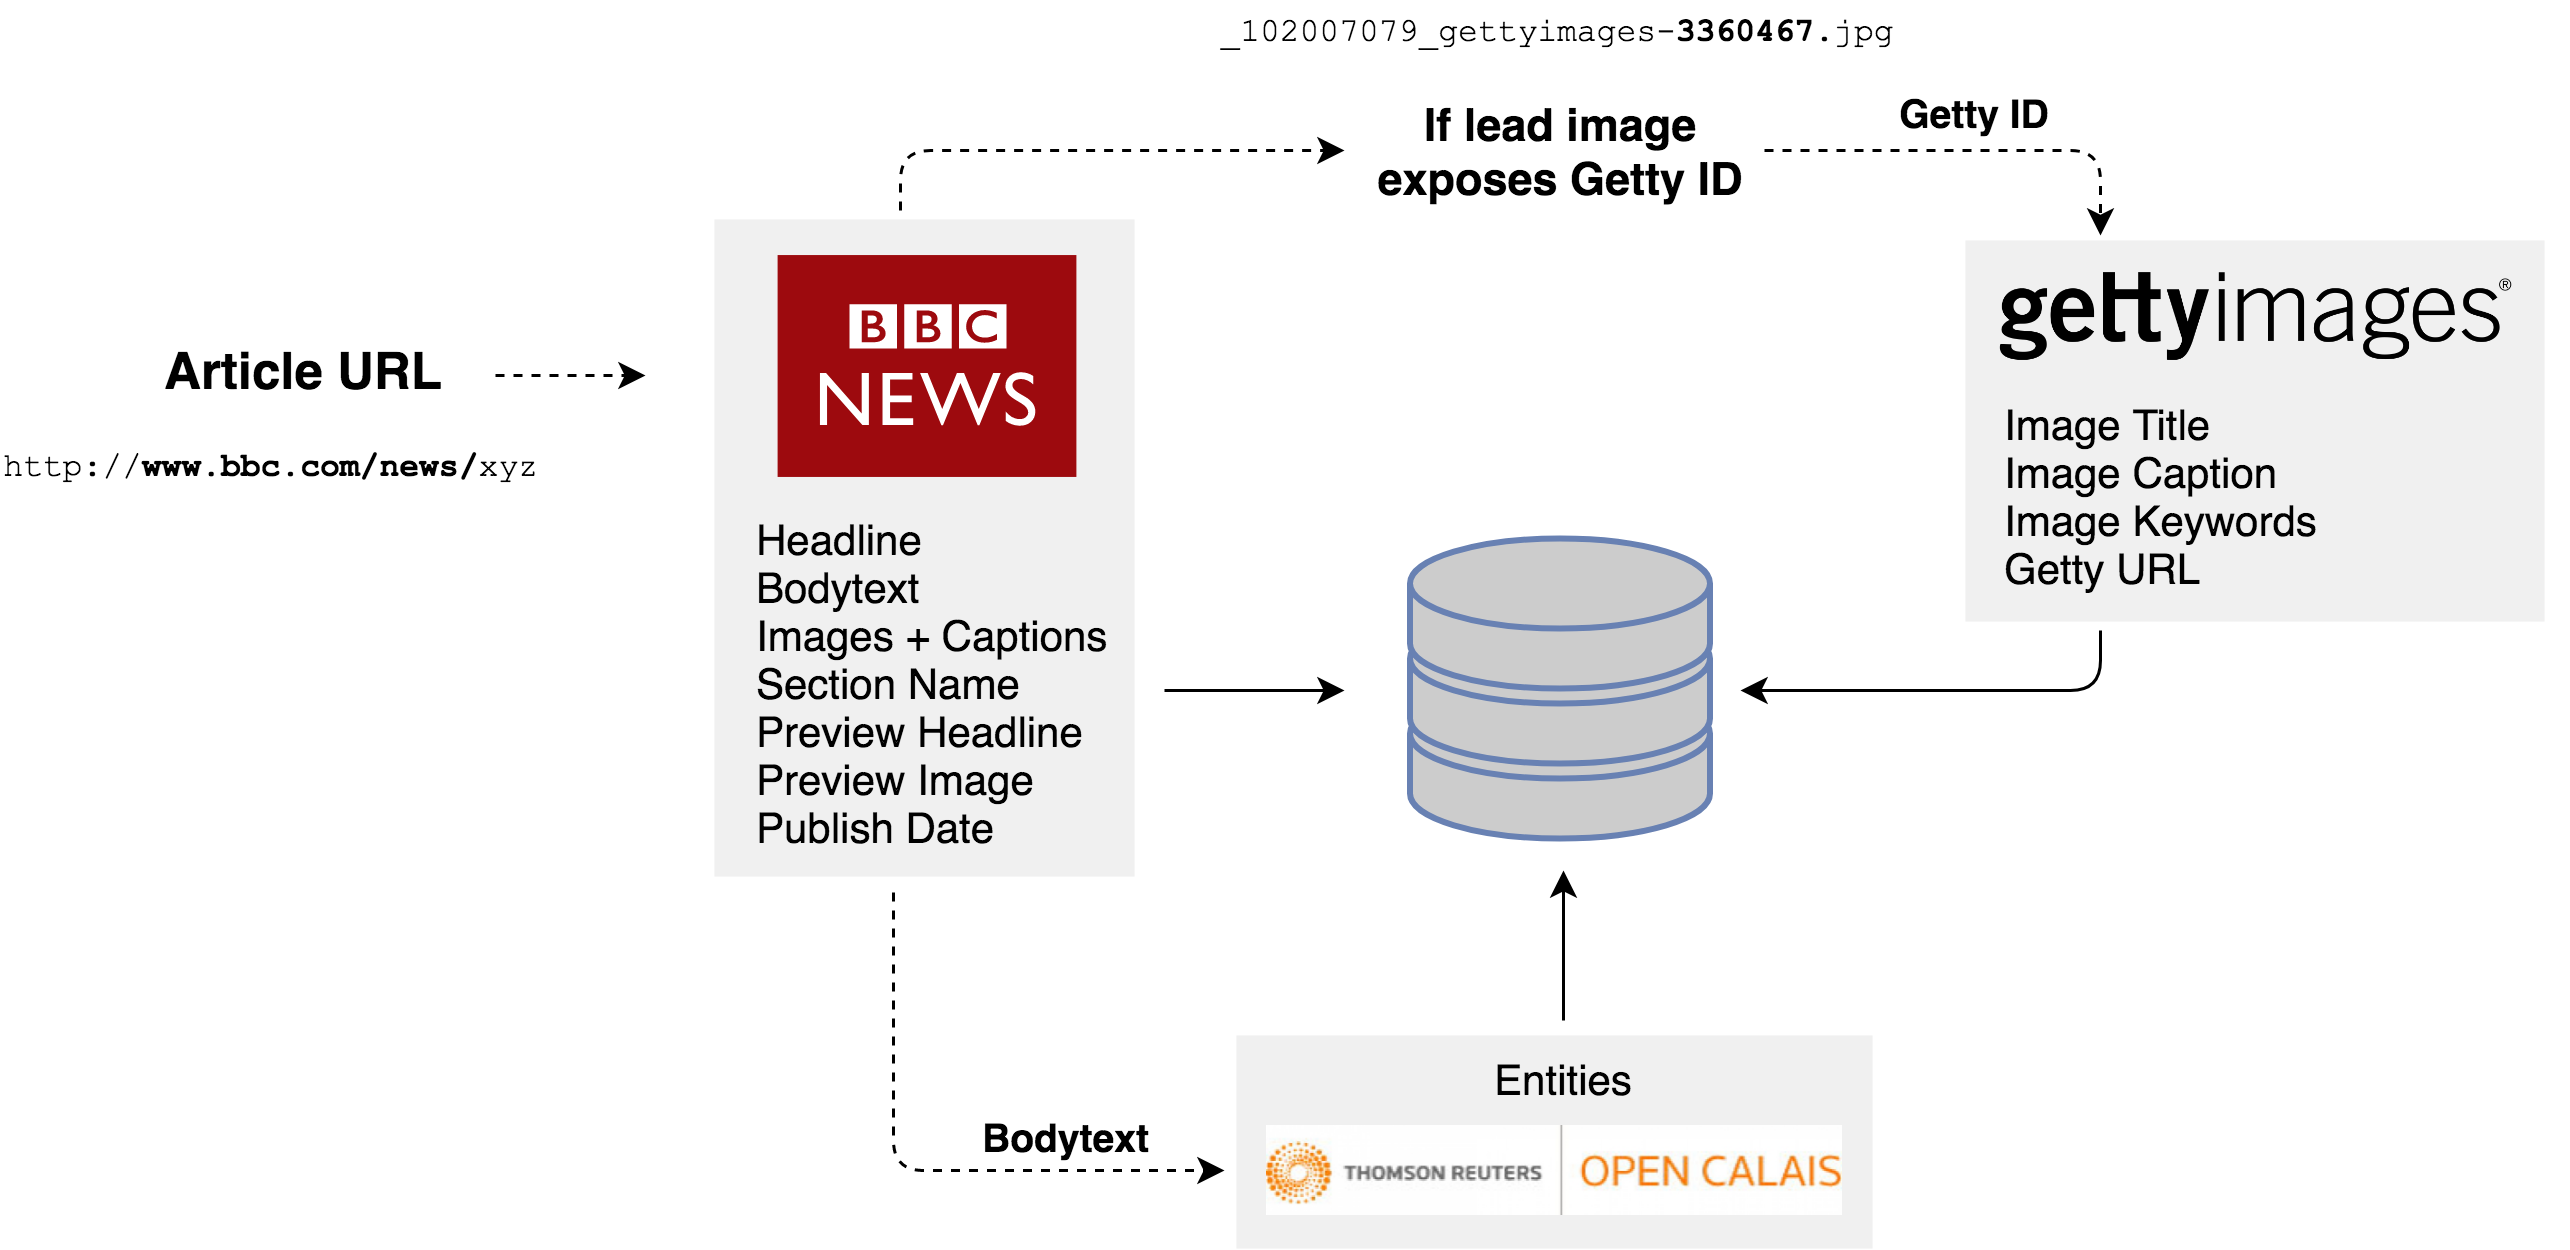
\includegraphics[width=\columnwidth]{picpic-scraper.png}
  \caption{Outline of the scraping procedure for one single article}
  \label{fig:picpic-scraper}
\end{figure}

The data set used for both training and evaluation of the system consists of two corpora. All images selected by the system are drawn from a large corpus published by the image agency \emph{Getty Images}. A collection of news articles was downloaded from the \emph{BBC News} website \cite{BBCBBCNews}.

Getty is particularly popular among media and news organisations worldwide and offers comprehensive coverage of contemporary news incidents, historical photography as well as stock photography. Using this corpus is therefore very close to a real-world application. Getty offers access to its image collection through an open web interface called "Getty Images API" \cite{GettyImagesAPIOverview} that is - with certain limitations - free to use. Besides this practical reason, Getty Images was chosen because it covers the whole range of possible images for news articles, from pictures of current events to symbolic pictures that illustrate abstract topics. From a developer's perspective, using the Getty API makes sense because it offers programmatic access to structured data ready to use and can be regarded as one instance of an arbitrary image database.

When news organisations publish an article, image meta data is usually not included. Knowing this meta data, however, is crucial for the proposed machine to learn from the selections human editors make, as will be seen in Section \ref{SystemTrain}. The challenge in collecting the article corpus was hence to find news articles that do not only contain an image by Getty but do additionally allow a conclusion about the original entry in Getty's database. It was found that many articles on the \emph{BBC News} website \cite{BBCBBCNews} do in fact expose the original IDs of the embedded Getty images via image URLs in the HTML documents. For example, in the following image URL

\begin{lstlisting}
_102007079_gettyimages-3360467.jpg
\end{lstlisting}

\noindent the Getty ID is \lstinline{3360467}. Likewise, BBC News is an applicable source with regards to contents: The website offers a vast collection of typical news articles every day. It focuses on reporting current events in a short and informative way and aims at a broad audience without a special interest. It publishes reports from all over the world and from many different topics, thereby closely resembling the coverage Getty offers.

With this knowledge in mind, a scraping application was designed that requests all articles from the BBC News website in a periodic fashion, stores them locally, checks for each article whether either the preview image or the first image in the article (i. e.  the lead image) exposes the original Getty ID, and if so requests the image meta data from the Getty API as well. The lead image restriction was imposed because on the BBC News website these are the images that come closest to what the proposed application is intended to select: One image that conveys the core message of the article.

The exemplified scraping work flow in Figure \ref{fig:picpic-scraper} shows that a third source was added: \emph{Thomson Reuters Open Calais} \cite{ThomsonReutersOpenCalais} is a web service that identifies persons, companies, events, products and many other entities in an unstructured text. By submitting the article text to Open Calais, some semantic information about the occurring entities could be stored alongside the plain article. More details on how Open Calais was used to improve the machine learning approach of this system will be presented in Sections \ref{SystemPreprocessCalais} and \ref{SystemClassificationML}.

The scraping application was deployed on 14 June 2018 and run each day on 9 a.m., 4 p.m. and 9 p.m. UTC. By 4 October 2018 it has collected 18,830 articles with their associated Open Calais entity tags. 1,578 of these articles contain a lead image that exposes the Getty ID, resulting in a set of training data consisting of approximately 500,000 terms and their associated features.

\subsection{Preprocessing an Article} \label{SystemPreprocess}

Processing an article written in natural language requires bringing structure to the unstructured text. Hence, this system contains a preprocessing component that turns the plain article text into a machine readable list of all the terms that occur in the text. Table \ref{table:term-examples} shows an example output of the preprocessor for a short piece of text. The exact steps the preprocessor performs are explained below.

\begin{table}[h!]
    \caption{Preprocessing result for "God helps those who help themselves."}
    \centering
    \begin{tabular}{|c|c|c|c|}
         \hline
         stemmed term & original terms & term frequency & first occurrence  \\
         \hline
         god          & God            & 1              & 0                 \\
         help         & helps, help    & 2              & 0.081             \\
         god help     & God helps      & 1              & 0                 \\
         help those who help & helps those who help & 1 & 0.081             \\
         \hline
    \end{tabular}
    \label{table:term-examples}
\end{table}

\paragraph{Tokenisation.} The first step is to turn the plain text, that is, a sequence of characters, into a sequence of words. This is achieved with a simple tokeniser that splits the original character sequence into substrings at every character that is neither an alphabetic letter, a digit nor an underscore. 

\paragraph{N-Gram Selection.} Since terms do not always consist of just one word, the preprocessor considers compounds consisting of up to four consecutive words as well, so called \emph{n-grams}. This is achieved by sliding a two, three and four word wide window over the previously generated list of words. However, only n-grams that do not overlap with a punctuation character (such as a full stop or a comma) are considered, i. e. n-grams must not exceed the borders of a clause. The n-grams are appended to the list of words.

\paragraph{Stopword Removal.} Many languages have words that convey little meaning on their own and can be left out from analysis, commonly referred to as "stopwords". In English these are mainly pronouns and particles such as "he", "themselves", "by", "when". The complete list of stopwords used in this system can be found in Appendix \ref{AppendixStopwords}. The preprocesor removes all these words from the word list, if they occur individually. Additionally, it removes any n-gram that starts or ends with a stopword, a procedure inspired by Hulth \cite{HulthImprovedKnowledge}.

\paragraph{Stemming.} In order to enable grouping of different inflections of the same word or closely related words, a procedure called "stemming" is applied to the complete word list. This refers to the reduction of words to their linguistic root. Porter's stemming algorithm \cite{Porter1980AnStripping} for the English language has proven to be reliable and effective and was hence chosen for this step.

\paragraph{Feature Assignment} After stemming, the preprocessor characterises each term with a set of features. The choice of features is a crucial part of the whole application, since these are the values the classifiers will use for deciding whether a term is a keyword or not. The features applied in this application are discussed in-depth in the following subsections.

\subsubsection{Features of a Term} \label{SystemPreprocessFeatures}

After the list of stemmed terms is assembled, many terms will occur more than once. Even though a simple measure, the frequency of a word does at least give some evidence about its importance for the text - an assumption fundamental to linguistic measures such as \emph{tf*idf} \cite{Salton1988Term-weightingRetrieval}. Manual benchmarks have largely confirmed this assumption for the BBC corpus on hand, which is why \textbf{term frequency} was included as the first, most basic feature for each term. The preprocessor eliminates duplicate words in the list by combining them to one list entry. It starts off by assigning a term frequency of 1 to each term and increments this count for each duplicate term it detects.

The most powerful term characteristic the manual benchmarks have revealed is the relative position at which a term occurs for the first time. The earlier a term is mentioned, the more important it seems to be for the story. This finding is not surprising, considering one of the basic writing techniques journalists use for presenting hard news: "placing the most important information at the beginning of the story, thus circumventing the reader's decision whether to continue or stop the reception." \cite[p. 501]{Pottker2003NewsAppear} This convention, commonly referred to as the "inverted pyramid" \cite[ibd.]{Pottker2003NewsAppear}, results in a decreasing amount of relevance over the course of a typical news article. Combined with term frequency, the \textbf{first occurrence} of a term rendered sufficiently good results for the statistical approach to be based on solely these two measures (see Section \ref{SystemClassificationStat}). In technical terms, this feature is implemented by searching the plain article text for the respective term and measuring the distance to the first character of the text relative to the total number of characters, i. e. a value of 0 refers to the first character in the article and 1 refers to the last.

Manual benchmarks were carried out for two other linguistic features, but the results were rather discouraging. A \textbf{part-of-speech} lookup in the WordNet database \cite{Fellbaum1998WordNet:Database} resulted in a 5-dimensional vector representing the number of nouns, verbs, adjectives, adverbs and other words in a term but did not reveal any pattern linked to image keywords in the benchmarks. It was therefore left out from this proposal. A feature called \textbf{paragraph type} was designed as a 4-dimensional vector that represents the number of times a term occurs in the headline, sub headlines, list items and regular paragraphs. Even though it seems likely that keywords occur in headlines and sub headlines, adding this feature actually blurred the results. BBC News uses sub headlines particularly often for inserting additional items into the article text that are not directly related, thus many words appeared to be keywords that were unrelated to the topic. All in all, the complications with this feature were more substantial than the benefits, which is why it was chosen to drop it.

\subsubsection{Enhancing Preprocessing with Semantic Tagging} \label{SystemPreprocessCalais}

One of the key difficulties in preprocessing the articles for term classification was the correct aggregation of terms that refer to one and the same thing. Consider for example the fictitious person "Jane Smith" who acts as a lawyer in an article: This person could be referred to with a range of different terms such as "Jane Smith", "Ms Smith", "Jane", "the lawyer", "the attorney", "the procurator", "lawyer Jane Smith" or simply "she". Some of these terms could be captured with naive approaches such as reacting to the keywords "Ms", "Mrs" and "Mr" or integrating sub terms into enclosing terms (e. g. "Jane" into "Jane Smith"). But never would suchlike approaches encompass all possible mentions.

It was therefore decided to enhance the preprocessing component with the automated semantic tagging system \emph{Open Calais}. Open Calais is a "web service that attaches intelligent metadata-tags to [...] unstructured content" \cite[p. 1]{ThomsonReuters2018ThomsonGuide}. The service offered by the news agency \emph{Thomson Reuters} processes natural language with an engine based on statistics, machine learning and other heuristics, and is free to use. The tags it assigns include the overall topics of a text, entities occurring in the text and relations between these entities. Entities can be persons, companies, organisations, countries, events and many more. The proposed system only makes use of Open Calais' entity detection, ignoring topics and relations.

\begin{table}[ht]
    \caption{Example for Open Calais entity detection}
    \centering
    \begin{tabular}{l p{10cm}}
        Input text: & \nohyphens{\emph{"\underline{Marty Balin} - \underline{the co-founder} of the psychedelic rock band \underline{Jefferson Airplane} - has died aged 76, \underline{his} family and publicist say. They did not specify the cause of death of \underline{the US musician}."}} \bigskip \\
        
        Detections: & \begin{tabular}{|l|l|l|}
         \hline
         \textbf{entity name} & \textbf{exact terms}        & \textbf{entity type}       \\
         \hline
         United States      & US                            & Country           \\
         \hline
         Jefferson Airplane & Jefferson Airplane            & MusicGroup        \\
         \hline
         Marty Balin        & \pbox{50cm}{\vspace{.2\baselineskip}Marty Balin\\the co-founder\\his\\the US musician\vspace{.3\baselineskip}} & Person            \\
         \hline
         co-founder & co-founder & Position \\
         \hline
         US musician & US musician & Position \\
         \hline
    \end{tabular}
    \end{tabular}
    \label{table:calais-example}
\end{table}

Adding this information to the system enables term aggregation way beyond the simple stemming explained above. As seen in Table \ref{table:calais-example}, Open Calais detects even small references to entities that consist of just one pronoun. This has three major benefits: Firstly, it enables a more detailed elimination of duplicate terms in the list, since each term that is detected as belonging to an entity can be merged with all other terms belonging to the same entity. Secondly, by exposing an entity name, Open Calais offers a way of detecting which occurrence of the term actually describes the entity in the most common fashion (and is hence best for using in the search term). And lastly, it enables a more precise specification of term frequency, counting not only direct mentions of an entity, but also paraphrased references to it.

Thomson Reuters does not disclose the exact methods Open Calais uses, but it clearly states that machine learning is involved \cite{ThomsonReuters2018ThomsonGuide}. This is at odds with the definition of the statistical approach in the presented system (see Section \ref{SystemClassificationStat}), which is why the additional aggregation described above is only applied in the machine learning approaches.

\bigskip

Adding Open Calais entity detection to the system enables another modification for the machine learning approaches: Since Open Calais does not only detect entities, but also assign an entity type, an optional term feature can be introduced. Those terms that were detected to be entities get assigned the additional feature \textbf{entity category}. This feature is meant to describe what "kind" of term one is dealing with, with the assumption in mind that some types of entities are better search terms than others (e. g. a person might be preferred to a country or an organisation's name). Open Calais knows 41 different entity types. In order to group together closely related entity types and to reduce complexity, they were combined into seven entity categories: Event, HumanProtagonist, OrganizationProtagonist, Position, Location, Product and Other. The exact grouping can be found in Appendix \ref{AppendixEntcats}. These group labels are then assigned as a feature value to each affected term.

\begin{table}[b]
    \caption{Entity categories for the terms in Table \ref{table:calais-example}}
    \centering
    \begin{tabular}{|c|c|c|}
        \hline
        \textbf{entity name} & \textbf{entity type} & \textbf{entity category} \\
        \hline
        United States & Country & Location \\
        Jefferson Airplane & MusicGroup & HumanProtagonist \\
        Marty Balin & Person & HumanProtagonist \\
        co-founder & Position & Position \\
        US musician & Position & Position \\
        \hline 
    \end{tabular}
    \label{table:entcat-example}
\end{table}

The actual benefit of adding these labels to the list of terms was not obvious in the manual benchmarks conducted before the implementation. However, their overall positive - yet not very strong - effect became visible in the evaluation of the implemented system that will be presented in Section \ref{Eval}. It remains to examine whether the information extracted by Open Calais can be used in a more advantageous manner than in this proposal. Some ideas towards deeper exploitation of semantic tagging can be found in Sections \ref{Limits} and \ref{Conclusion}.

\subsection{Training Neural Networks} \label{SystemTrain}

\begin{figure}[h]
  %% Datei auf ganze Breite des Texts vergrößert
  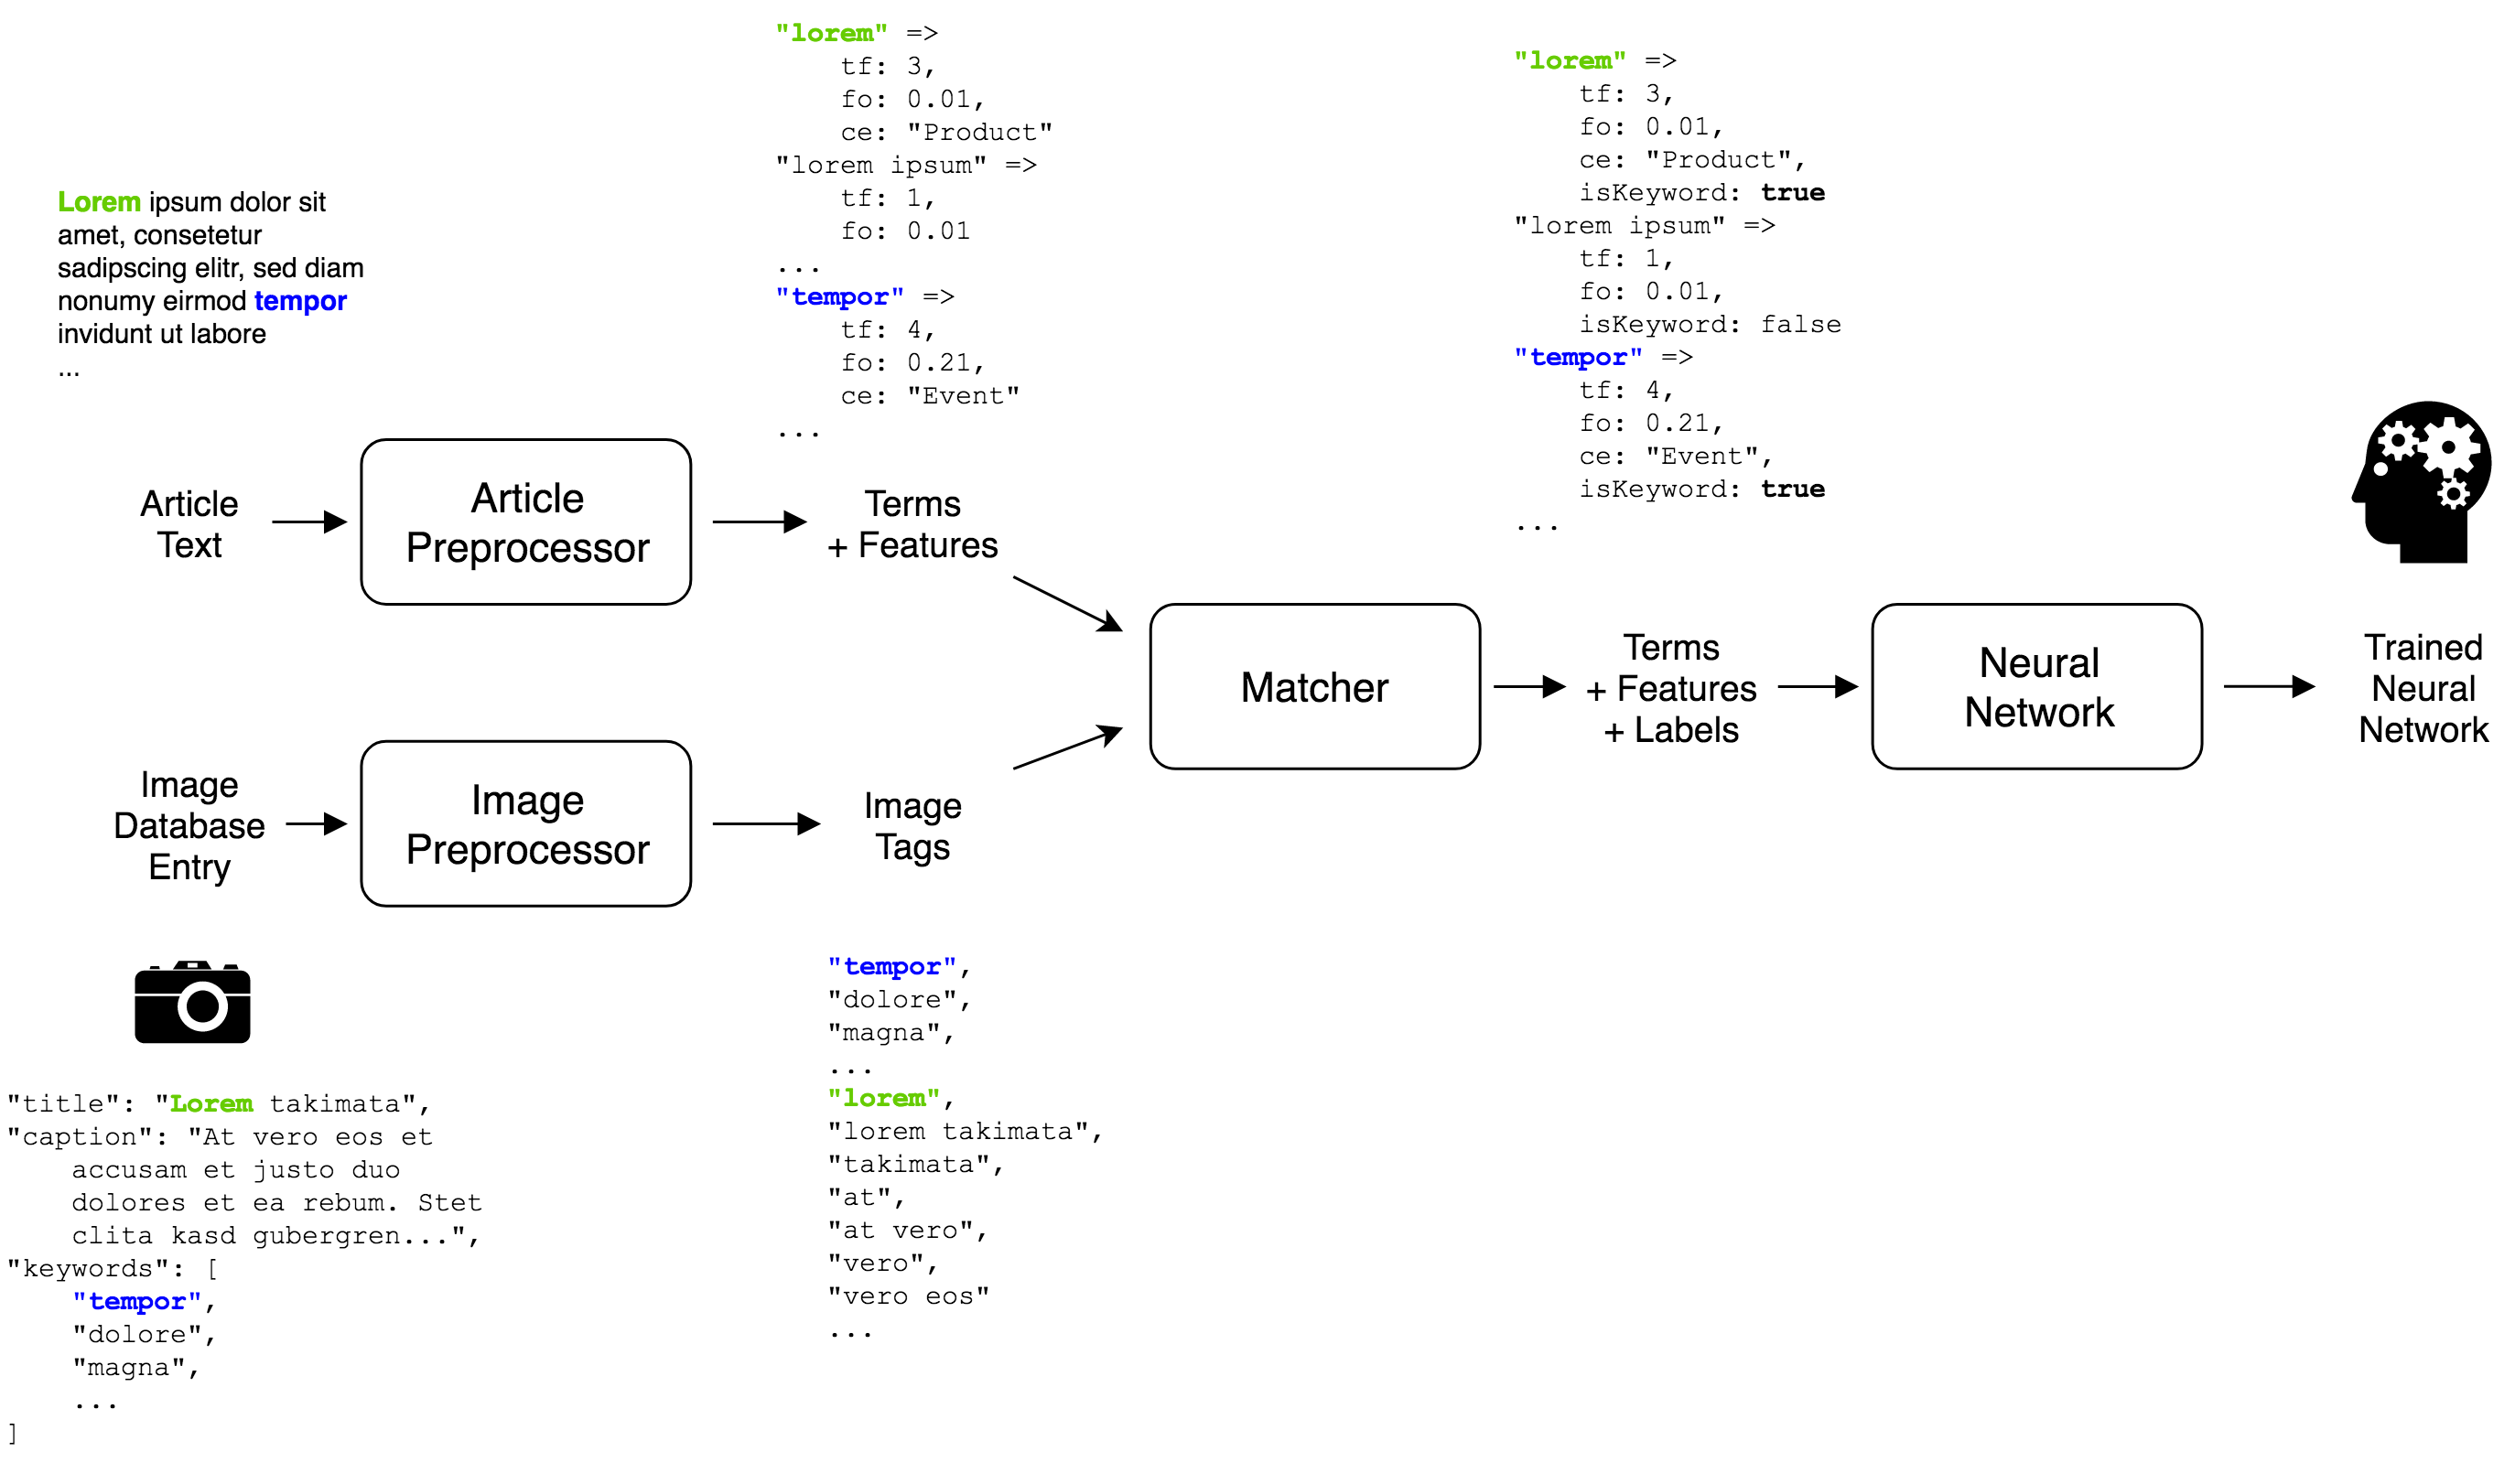
\includegraphics[width=\columnwidth]{picpic-training.png}
  \caption{Outline of the training pipeline}
  \label{fig:picpic-training}
\end{figure}

\subsubsection{Preprocessing an Image for Training} \label{SystemTrainPreprocess}
\subsubsection{Generating Training Data} \label{SystemTrainGenerate}
\subsubsection{Training the Networks} \label{SystemTrainTrain}

\subsection{Term Classification} \label{SystemClassification}
\subsubsection{Statistics Based Approach} \label{SystemClassificationStat}
\subsubsection{Machine Learning Based Approach} \label{SystemClassificationML}

\subsection{Image Query} \label{SystemQuery}

%______________________________________________________________________

\cleardoublepage

\section{Evaluation} \label{Eval}

\subsection{Factual Correctness as a Measure for System Performance} \label{EvalFacts}

\subsection{Evaluation Design} \label{EvalDesign}

\subsection{Evaluation Results} \label{EvalResults}

%______________________________________________________________________

\cleardoublepage

\section{Limitations} \label{Limits}

\subsection{System Limitations} \label{LimitsSystem}

\subsection{Research Design Limitations} \label{LimitsEval}

%______________________________________________________________________

\cleardoublepage

\section{Conclusion} \label{Conclusion}

%______________________________________________________________________

\iffalse

% Der Befehl \cleardoublepage erscheint nur vor \section, nicht vor
% den "kleineren" Gliederungsbefehlen wie \subsection!
\cleardoublepage % Neue rechte Seite anfangen
\section{Example Section}

\begin{figure}%[btph]
  %% Datei ``beispielbild.eps'' oder ``beispielbild.png'', zentriert
  %\begin{center}\includegraphics{beispielbild}\end{center}

  %% Datei auf 8cm Breite verkleinert/vergrößert
  %\includegraphics[width=8cm]{beispielbild}
  %% Datei auf ganze Breite des Texts vergrößert
  %\includegraphics[width=\columnwidth]{beispielbild}
  %% Datei auf 60% der Textbreite verkleinert/vergrößert
  %\includegraphics[width=.6\columnwidth]{beispielbild}
  %% Weitere Optionen (Ausschnitt, drehen etc.) in der Doku zum graphicx-Paket

  \begin{center}\LARGE [BILD]\end{center}
  \caption{Bildunterschrift}
  \label{fig:beispielbild}
\end{figure}


Siehe Abbildung \ref{fig:beispielbild} oder einschlägige Literatur, z.B.
\cite[Seite 6]{Brill1992ATagger} oder \cite{Porter1980AnStripping}.

\bigskip % Größerer Abstand zum vorherigen Absatz
\textbf{Hinweis:} Die Verweise im generierten PDF (HTTP-Links, Verweise auf Kapitel oder Bilder) sind leicht eingefärbt. Wer das nicht will, z.B. weil es die Druckkosten erhöht, kann am Anfang des Dokuments \texttt{linkcolor} usw. auf ``black'' setzen.


\subsection{Medien}

\begin{figure}
  \begin{center}\LARGE [BILD]\end{center}
  \caption{Noch ein Bild}
  \label{fig:beispielbild2}
\end{figure}

\begin{itemize}
  \item Gesellschaftliche Medien
  \item Technische Medien
\end{itemize}


\subsection{Informatik}


\subsection{Medieninformatik}

\begin{description}
  \item[Medienwirkung:] Ein Spezialfach der Kommunikationswissenschaft. Für das erfolgreiche Studium des Anwendungsfachs Mediengestaltung ist eine künstlerische Begabung erforderlich.
  \item[Medienwirtschaft:] Ein Spezialfach der Betriebswirtschaftslehre
  \item[Mediengestaltung:] Ein Spezialfach der Kunstwissenschaft
\end{description}

\subsubsection{Was Sie schon immer wissen wollten, aber nie zu fragen
  wagten}

\paragraph{Überschrift}
Diese Überschrift erscheint fettgedruckt am Anfang des Absatzes.

\subsubsection{Was Sie nicht wissen wollten}

Text text textextext\footnote{Oder so ähnlich}.

\fi

%\_____________________________________________________________________

\cleardoublepage
\begin{appendix}

\section{Source Code} \label{AppendixCode}

The proposed system has been implemented in JavaScript for Node.js for research reasons. It consists of four open source projects that can either be found on the CD attached to the printed version of this thesis or under the links provided below.

\begin{table}[h]
    \centering
    \begin{tabular}{|c|p{4.5cm}|c|}
        \hline
        \textbf{Project Name} & \textbf{Description} & \textbf{URL} \\
        \hline
        gettygetter & Scraping application for collecting data from BBC News, Getty Images and Open Calais & \url{https://github.com/mgschoen/gettygetter} \\
        \hline
        picpic-core & Collection of tools for preprocessing, keyword extraction and training of neural networks & \url{https://github.com/mgschoen/picpic-core} \\
        \hline
        picpic-api & Public REST interface that applies the image selection pipeline to the corpus collected with gettygetter & \url{https://github.com/mgschoen/picpic-api} \\
        \hline
        picpic-explorer & Statically served web frontend for interacting with picpic-api & \url{https://github.com/mgschoen/picpic-explorer} \\
        \hline
    \end{tabular}
    \label{table:source-code}
\end{table}

\clearpage

\section{List of Stopwords} \label{AppendixStopwords}

\emph{The character "," in the following list denotes a word separator.}

\bigskip

\noindent about, above, after, again, all, also, am, an, and, another, any, are, as, at, be, because, been, before, being, below, between, both, but, by, came, can, cannot, come, could, did, do, does, doing, during, each, few, for, from, further, get, got, has, had, he, have, her, here, him, himself, his, how, if, in, into, is, it, its, itself, like, make, many, me, might, more, most, much, must, my, myself, never, new, now, of, on, only, or, other, our, ours, ourselves, out, over, own, said, same, see, she, should, since, so, some, still, such, take, than, that, the, their, theirs, them, themselves, then, there, these, they, this, those, through, to, too, under, until, up, very, was, way, we, well, were, what, where, when, which, while, who, whom, with, would, why, you, your, yours, yourself, a, b, c, d, e, f, g, h, i, j, k, l, m, n, o, p, q, r, s, t, u, v, w, x, y, z, \$, 1, 2, 3, 4, 5, 6, 7, 8, 9, 0, \_

\clearpage

\section{Grouping of Open Calais Entity Types} \label{AppendixEntcats}

\begin{table}[h!]
    \centering
    \begin{tabular}{|c|p{10cm}|}
        \hline
        \textbf{Group}          & \textbf{Associated Entity Types} \\
        \hline
        Event                   & \nohyphens{Anniversary, Date, EntertainmentAwardEvent, Holiday, PoliticalEvent, SportsEvent, SportsGame, SportsLeague, TVShow} \\
        \hline
        HumanProtagonist        & Editor, Journalist, MusicGroup, Person \\
        \hline
        OrganizationProtagonist & Company, Organization \\
        \hline
        Position                & Position \\
        \hline
        Location                & \nohyphens{City, Continent, Country, Facility, NaturalFeature, ProvinceOrState, Region} \\
        \hline
        Product                 & \nohyphens{Movie, MusicAlbum, OperatingSystem, PharmaceuticalDrug, Product, ProgrammingLanguage, PublishedMedium, RadioProgram, RadioStation, Technology, TVShow, TVStation} \\
        \hline
        Other                   & \nohyphens{EmailAddress, FaxNumber, IndustryTerm, MarketIndex, MedicalCondition, MedicalTreatment, PhoneNumber, URL} \\
        \hline
    \end{tabular}
    \label{table:entity-groups}
\end{table}

\end{appendix}

%\_____________________________________________________________________

\cleardoublepage
\fancyhead[LE,RO,LO,RE]{} % Keine Kopfzeile mehr oben auf jeder Seite
\section*{Contents of the Attached CD}
%______________________________________________________________________

\cleardoublepage
%\begin{thebibliography}{99}

%\bibitem{Ivory01}

%  M.\ Y.\ Ivory, M.\ Hearts:
%  \href{http://www.ischool.washington.edu/myivory/thesis/thesis.pdf}{%
%    An Empirical Foundation for Automated Web Interface Evaluation}.
%  Ph.D. thesis, University of California at Berkeley, 2001


%\cleardoublepage
%\hspace{-\leftmargin}{\Large\bfseries Web-Referenzen} % Wüster Hack %-|

%\bibitem{NielsenAlertbox}

%  J.\ Nielsen: Alertbox: Current Issues in Web Usability
%  \url{http://useit.com/alertbox/}, accessed April~24, 2005.

%\end{thebibliography}

\bibliographystyle{plain}
\bibliography{mendeley_v2}

\end{document}
